\documentclass[a4paper,12pt]{article}
\usepackage[indonesian]{babel}
\usepackage{graphicx}
\usepackage{multirow}
\usepackage{enumitem}
\usepackage{listings}
\usepackage{wrapfig}
\usepackage[T1]{fontenc}
\usepackage{inconsolata}
\usepackage{lipsum}
\usepackage{adjustbox}


\usepackage{color}
\usepackage[table]{xcolor}
\definecolor{mygreen}{rgb}{0,0.6,0}
\definecolor{mygray}{rgb}{0.5,0.5,0.5}
\definecolor{mymauve}{rgb}{0.58,0,0.82}
\lstset{%
    language=java,
    showstringspaces=false,          % Prevent tex replacing space to bracket in code
    frame=single,                    % Set frame around code
    backgroundcolor=\color{white},   % choose the background color
    basicstyle=\footnotesize,        % size of fonts used for the code
    breaklines=true,                 % automatic line breaking only at whitespace
    captionpos=b,                    % sets the caption-position to bottom
    commentstyle=\color{mygreen},    % comment style
    keywordstyle=\color{blue},       % keyword style
    stringstyle=\color{mymauve},     % string literal style
}

\graphicspath{ {./img/} }
\begin{document}
\title{ {\Large Laporan Praktikum}\\ Algoritma dan Pemrograman Lanjut\\{\Large Pertemuan 11}}

\author{Aldzikri Dwijayanto Prathama
    \\195410189
    \\Informatika}
\makeatletter
\begin{titlepage}
    \begin{center}
        {\huge \bfseries \@title}\\[14ex]
        
\includegraphics[scale=.8]{logo}\\[4ex]
        {\large \@author}\\[12ex]
        {\large \bfseries {SEKOLAH TINGGI MANAJEMEN INFORMATIKA DAN KOMPUTER
            AKAKOM YOGYAKARTA}}
    \end{center}


%{\large \@date}
\end{titlepage}
\makeatother
%\maketitle
\newpage
\tableofcontents
\newpage

\section{Tujuan}
Mahasiswa dapat memahami dan menyelesaikan kasus dengan rekursif.
\section{Teori}
\paragraph{}
Program-program yang telah kita bahas sejauh ini umumnya disusun sebagai method yang
memanggil satu sama lain secara hierarkis. Untuk beberapa masalah, ada baiknya memanggil
method itu sendiri. Method yang dikenal sebagai method rekursif. Method rekursif dapat
memanggil dirinya baik secara langsung atau tidak langsung melalui method lain. Konsep rekursif. Pendekatan pemecahan masalah rekursif memiliki sejumlah elemen yang sama. Ketika
method rekursif dipanggil untuk memecahkan masalah, sebenarnya hanya mampu
menyelesaikan kasus yang paling sederhana, atau kasus dasar. Jika method ini disebut dengan
kasus dasar, method itu mengembalikan hasil. Jika method ini disebut dengan masalah yang
lebih kompleks, method tersebut biasanya membagi masalah menjadi dua bagian konseptual

— bagian yang diketahui cara melakukannya dan bagian yang tidak diketahui bagaimana
melakukannya. Untuk membuat rekursi menjadi layak, bagian yang terakhir harus menyerupai
masalah aslinya, tetapi versi yang sedikit lebih sederhana atau lebih kecil. Karena masalah
baru ini terlihat seperti masalah asli, method ini memanggil salinan baru dari dirinya untuk
bekerja pada masalah yang lebih kecil — ini disebut sebagai panggilan rekursif dan juga
disebut langkah rekursi. Langkah rekursi biasanya mencakup pernyataan pengembalian, karena hasilnya akan digabungkan dengan bagian dari masalah yang diketahui method untuk
menyelesaikan untuk membentuk hasil yang akan diteruskan kembali ke penelepon asli. Langkah rekursi dijalankan sementara pemanggilan method asli masih aktif (mis., Belum
selesai dieksekusi). Ini dapat menghasilkan lebih banyak panggilan rekursif karena method ini
membagi setiap sub-masalah baru menjadi dua bagian konseptual. Agar rekursi akhirnya
berakhir, setiap kali method memanggil dirinya sendiri dengan versi yang lebih sederhana dari
masalah aslinya, urutan masalah yang lebih kecil dan lebih kecil harus menyatu pada kasus
dasar. Ketika method mengenali kasus dasar, itu mengembalikan hasil ke salinan method
sebelumnya. Urutan pengembalian terjadi sampai pemanggilan method asli mengembalikan
hasil akhir ke pemanggil. Method rekursif dapat memanggil method lain, yang pada gilirannya membuat panggilan
kembali ke method rekursif. Ini dikenal sebagai panggilan rekursif tidak langsung atau rekursi
tidak langsung. Misalnya, method A memanggil method B, yang membuat panggilan kembali
ke method A. Ini masih rekursi, karena panggilan kedua ke method A dilakukan saat panggilan
pertama ke method A aktif — yaitu panggilan pertama ke method A belum selesai dieksekusi
(karena sedang menunggu method B untuk mengembalikan hasilnya) dan belum kembali ke
pemanggil asli method A. Untuk lebih memahami konsep rekursi, mari kita lihat contoh yang
cukup akrab bagi pengguna komputer — definisi rekursif direktori pada komputer. Komputer
biasanya menyimpan file terkait dalam direktori. Direktori dapat kosong, dapat berisi file dan
/ atau dapat berisi direktori lain (biasanya disebut sebagai subdirektori). Masing-masing
subdirektori ini, pada gilirannya, dapat juga berisi file dan direktori. Jika kita ingin membuat
daftar setiap file dalam direktori (termasuk semua file dalam subdirektori direktori), kita
perlu membuat method yang pertama-tama mendaftar file direktori awal, kemudian
membuat panggilan rekursif untuk membuat daftar file di masing-masing subdirektori
direktori itu. Kasus dasar terjadi ketika direktori tercapai yang tidak mengandung subdirektori. Pada titik ini, semua file dalam direktori asli telah terdaftar dan tidak perlu rekursi lebih
lanjut. (Sumber : Deitel, Deitel edisi 9)
Dalam pemrograman, rekursif dapat diimplementasikan pada method. Syarat supaya method
rekursi dapat terjadi adalah harus ada kondisi dimana pemanggilan terhadap method itu
sendiri berakhir.
\newpage

\section{Pembahasan}
\subsection{Praktik}
\subsubsection{Praktik 1}
\begin{lstlisting}
public class FaktorialRekursif {

    public static long faktorial(long N) {
        if (N <= 1)
            return 1;
        else
            return N * faktorial(N -1);
    }

    public static void main(String[] args) {
        System.out.println("Faktorial 5 = " + faktorial(5));
    }
}
\end{lstlisting}

Program tersebut memiliki dua buah fungsi, fungsi faktorial berisi rekursif, yang berfungsi untuk menghitung faktorial,
jika nilai N bernilai kurang dari 1, maka fungsi akan mengembalikan nilai 1, jika tidak maka dilakukan operasi rekursif
. Lalu fungsi main berfungsi untuk input, dan memanggil fungsi.

\begin{center}
    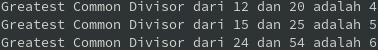
\includegraphics[scale=1]{1.png} 
\end{center}

\subsubsection{Praktik 2}
\begin{lstlisting}
public class FibonacciRekursif {

    public static long fibonacci(long N) {
        if ((N==0) || (N==1))
            return N;
        else
            return fibonacci(N-1) + fibonacci(N-2);
    }

    public static void main(String[] args) {
        System.out.println("Deret fibonacci dengan N = 3");
        for (int i=0; i<=3; i++){
            if (i<3)
                System.out.print(fibonacci(i) + ", ");
            else
                System.out.println(fibonacci(i));
        }
    }
}
\end{lstlisting}
Program tersebut memiliki dua buah fungsi, fungsi fibonacci berisi rekursif, yang berfungsi untuk mencetak bilangan ke
layar, jika N tidak bernilai 1 atau 0, maka program akan menjalankan operasi rekursif. Lalu fungsi main berfungsi untuk input, dan memanggil fungsi.

\begin{center}
    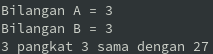
\includegraphics[scale=1]{2.png} 
\end{center}


\subsubsection{Praktik 3}
\begin{lstlisting}
public class FaktorialRekursifA {

    public static long faktorial(long N) {
        long bil = N;
        if (N <= 1) {
            bil = 1;
        }
        else {
            bil = N * faktorial(N -1);
        }
        System.out.print(bil + ", ");
        return bil;
    }

    public static void main(String[] args) {
        System.out.println("Faktorial 5 = " + faktorial(5));
    }
}
\end{lstlisting}
Program pada praktik 3 merupakan program dari praktik 1 sehingga program dapat menampilkan semua hasil faktorial dari
bilangan-bilangan sebelumnya. Pada program ini ditambahkan variabel bil, dan pernyataan print untuk menampilkan semua
hasil faktorial bilangan-bilangan sebelumnya.

\begin{center}
    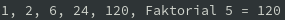
\includegraphics[scale=1]{3.png} 
\end{center}

\newpage

\subsection{Latihan}
\subsubsection{Latihan 1}
\begin{lstlisting}
import java.util.Scanner;

public class PangkatRekursif {

    private static int pangkat(int A, int B) {
        if (B==0) {
            return 1;
        } else {
            return A * pangkat(A,B-1);
        }
    }

    public static void main(String[] args) {
        Scanner in = new Scanner(System.in);
        System.out.print("Bilangan A = ");
        int bilA = in.nextInt();
        System.out.print("Bilangan B = ");
        int bilB = in.nextInt();
        in.close();
        System.out.println(bilA + " pangkat " + bilB + " sama dengan "+pangkat(bilA,bilB));
    }

}
\end{lstlisting}

Program pada Latihan pertama adalah program untuk menghitung pangkat dengan method rekursif. Pada method pertama jika
nilai B adalah 0, maka method akan mengembalikan nilai 1, jika tidak maka method akan menjalankan operasi rekursif.

\begin{center}
    
\includegraphics[scale=1]{4.png} 
\end{center}

\subsubsection{Praktik 2}
\begin{lstlisting}
public class GreatestCommonDivisor {
    public static int gcd(int X, int Y){
    	if (Y == 0) {
    		return X;
    	}else{
    		return gcd(Y, X%Y);
    	}
    }
    public static void main(String[] args) {
    	System.out.println("Greatest Common Divisor dari 12 dan 20 adalah " + gcd(12,20));
    	System.out.println("Greatest Common Divisor dari 15 dan 25 adalah " + gcd(15,25));
    	System.out.println("Greatest Common Divisor dari 24 dan 54 adalah " + gcd(24,54));
    }
}
\end{lstlisting}
Program pada latihan 2 adalah mencari FPB dari dua bilangan, pada method pertama jika Y bernilai 0, maka method akan
mengembalikan nilai X, jika tidak maka program akan menjalankan rekursif, dengan parameter X dengan input dari Y, dan Y
dengan input dari operasi modulus X, dengan Y.

\begin{center}
    
\includegraphics[scale=1]{5.png} 
\end{center}

\newpage

\subsection{Tugas}
\begin{lstlisting}
import java.util.Scanner;
class PalindromeCheck
{
    public static boolean isPal(String s)
    {   
        if(s.length() == 0 || s.length() == 1)
            return true; 
        if(s.charAt(0) == s.charAt(s.length()-1))
        return isPal(s.substring(1, s.length()-1));

        return false;
    }

    public static void main(String[]args)
    {
        Scanner scanner = new Scanner(System.in);
        System.out.println("Enter the String for check:");
        String string = scanner.nextLine();
        if(isPal(string))
            System.out.println(string + " is a palindrome");
        else
            System.out.println(string + " is not a palindrome");
    }
}
\end{lstlisting}
Program untuk tugas adalah program yang berfungsi untuk menngecek apakah sebuah kata berbentuk palindrom atau bukan.
Pada fungsi pertama yaitu isPal dilakukan pengecekan antara karakter yang berada di depan dan di belakang, pengecekan
dildilakukan sampai ke tengah kata. Lalu pada method main berfungsi untuk memasukkan kata, dan mencetak hasil ke layar.

\begin{center}
    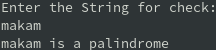
\includegraphics[scale=1]{6a.png} 
    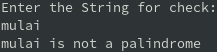
\includegraphics[scale=1]{6b.png} 
\end{center}


\newpage

\section{Kesimpulan}
Setelah praktik Mahasiswa dapat memahami dan menyelesaikan kasus dengan rekursif.

\end{document}
